%                **** IMPORTANT NOTICE *****
% This LaTeX file has been automatically produced by ProTeX v. 1.1
% Any changes made to this file will likely be lost next time
% this file is regenerated from its source. Send questions 
% to Arlindo da Silva, dasilva@gsfc.nasa.gov
 
\setlength{\oldparskip}{\parskip}
\setlength{\parskip}{1.5ex}
\setlength{\oldparindent}{\parindent}
\setlength{\parindent}{0pt}
\setlength{\oldbaselineskip}{\baselineskip}
\setlength{\baselineskip}{11pt}
 
%--------------------- SHORT-HAND MACROS ----------------------
\def\bv{\begin{verbatim}}
\def\ev{\end{verbatim}}
\def\be{\begin{equation}}
\def\ee{\end{equation}}
\def\bea{\begin{eqnarray}}
\def\eea{\end{eqnarray}}
\def\bi{\begin{itemize}}
\def\ei{\end{itemize}}
\def\bn{\begin{enumerate}}
\def\en{\end{enumerate}}
\def\bd{\begin{description}}
\def\ed{\end{description}}
\def\({\left (}
\def\){\right )}
\def\[{\left [}
\def\]{\right ]}
\def\<{\left  \langle}
\def\>{\right \rangle}
\def\cI{{\cal I}}
\def\diag{\mathop{\rm diag}}
\def\tr{\mathop{\rm tr}}
%-------------------------------------------------------------

\markboth{Left}{Source File: ESMF\_XGridSparseMatEx.F90,  Date: Tue May  5 20:59:57 MDT 2020
}

 
%/////////////////////////////////////////////////////////////

  \subsubsection{Create an XGrid from user input data then use it for regridding}
  \label{sec:xgrid:usage:xgrid_createfromsparsemat}
  
   Alternatively, XGrid can be created from Grids on either side,
   area and centroid information of XGrid cells, sparse matrix matmul information.
   The functionalities provided by the
   XGrid object is constrained by the user supplied input during its creation time.
  
   In this example, we will set up a simple XGrid from overlapping Grids on
   either side of the XGrid. Then we perform a flux exchange from one side
   to the other side of the XGrid. The Grids are laid out in the following figure:
  \begin{center}
  \begin{figure}
  \center
  \scalebox{0.6}{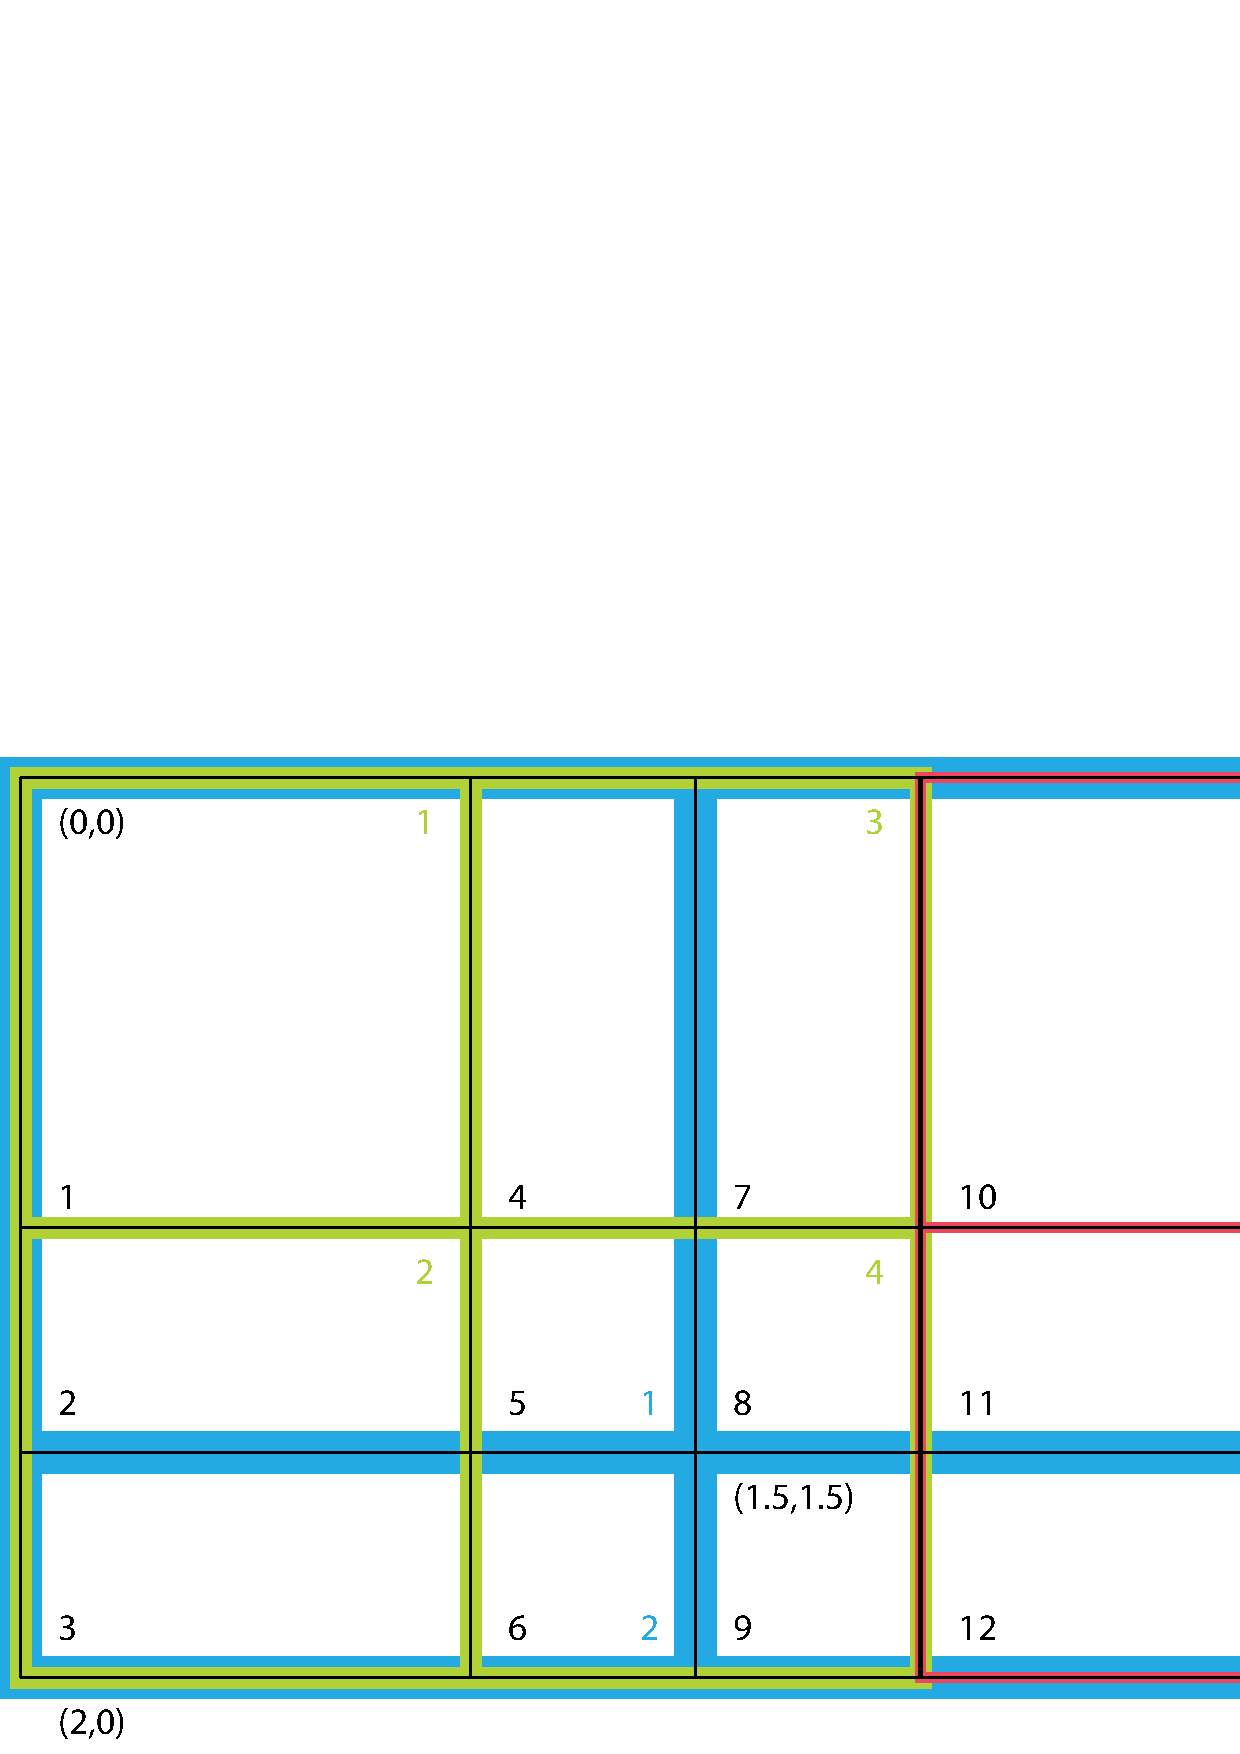
\includegraphics{XGridEx1}}
  \caption{Grid layout for simple XGrid creation example. Overlapping of 3 Grids
  (Green 2x2, Red 2x1, Blue 2x2). Green and red Grids on side A, blue Grid on side
  B, black indicates the resulting XGrid. Color coded sequence indices are shown.
  Physical coordinates are the tuples in parenthesis, e.g. at the four
  corners of rectangular computational domain.}
  \label{fig:xgridsimple}
  \end{figure}
  \end{center}
  
   We start by creating the Grids on both sides and associate coordinates with
   the Grids. For details of Grid creation and coordinate use, please refer to
   Grid class documentation. 
%/////////////////////////////////////////////////////////////

 \begin{verbatim}
    sideA(1) = ESMF_GridCreateNoPeriDim(minIndex=(/1,1/), maxIndex=(/2,2/), &
        coordDep1=(/1/), &
        coordDep2=(/2/), &
        name='source Grid 1 on side A', rc=localrc)
 
\end{verbatim}
 
%/////////////////////////////////////////////////////////////

 \begin{verbatim}
    sideA(2) = ESMF_GridCreateNoPeriDim(minIndex=(/1,1/), maxIndex=(/2,1/), &
        coordDep1=(/1/), &
        coordDep2=(/2/), &
        name='source Grid 2 on side A', rc=localrc)
 
\end{verbatim}
 
%/////////////////////////////////////////////////////////////

 \begin{verbatim}
    do i = 1, 2
        call ESMF_GridAddCoord(sideA(i), staggerloc=ESMF_STAGGERLOC_CENTER, &
            rc=localrc)
 
\end{verbatim}
 
%/////////////////////////////////////////////////////////////

 \begin{verbatim}
    enddo
 
\end{verbatim}
 
%/////////////////////////////////////////////////////////////

   Coordinate for the Grids on sideA, refer to the Grid layout diagram for the
   interpretation of the coordinate values: 
%/////////////////////////////////////////////////////////////

 \begin{verbatim}
    ! SideA first grid
    centroidA1X=(/0.5, 1.5/)
    centroidA1Y=(/0.5, 1.5/)
    call ESMF_GridGetCoord(sideA(1), localDE=0, &
        staggerLoc=ESMF_STAGGERLOC_CENTER, coordDim=1, &
        farrayPtr=coordX, rc=localrc)
 
\end{verbatim}
 
%/////////////////////////////////////////////////////////////

 \begin{verbatim}
    coordX = centroidA1X
    call ESMF_GridGetCoord(sideA(1), localDE=0, &
        staggerLoc=ESMF_STAGGERLOC_CENTER, coordDim=2, &
        farrayPtr=coordY, rc=localrc)
 
\end{verbatim}
 
%/////////////////////////////////////////////////////////////

 \begin{verbatim}
    coordY = centroidA1Y

    ! SideA second grid
    centroidA2X=(/0.5, 1.5/)
    centroidA2Y=(/2.5/)
    call ESMF_GridGetCoord(sideA(2), localDE=0, &
        staggerLoc=ESMF_STAGGERLOC_CENTER, coordDim=1, &
        farrayPtr=coordX, rc=localrc)
 
\end{verbatim}
 
%/////////////////////////////////////////////////////////////

 \begin{verbatim}
    coordX = centroidA2X
    call ESMF_GridGetCoord(sideA(2), localDE=0, &
        staggerLoc=ESMF_STAGGERLOC_CENTER, coordDim=2, &
        farrayPtr=coordY, rc=localrc)
 
\end{verbatim}
 
%/////////////////////////////////////////////////////////////

 \begin{verbatim}
    coordY = centroidA2Y
 
\end{verbatim}
 
%/////////////////////////////////////////////////////////////

   Create the destination grid on side B, only one Grid exists on side B. Also associate
   coordinate with the Grid: 
%/////////////////////////////////////////////////////////////

 \begin{verbatim}
    sideB(1) = ESMF_GridCreateNoPeriDim(minIndex=(/1,1/), maxIndex=(/2,2/), &
        coordDep1=(/1/), coordDep2=(/2/), &
        name='destination Grid on side B', rc=localrc)
 
\end{verbatim}
 
%/////////////////////////////////////////////////////////////

 \begin{verbatim}
    do i = 1, 1
        call ESMF_GridAddCoord(sideB(i), staggerloc=ESMF_STAGGERLOC_CENTER, &
            rc=localrc)
 
\end{verbatim}
 
%/////////////////////////////////////////////////////////////

 \begin{verbatim}
    enddo

    ! SideB grid
    centroidBX=(/0.75, 1.75/)
    centroidBY=(/0.75, 2.25/)
    call ESMF_GridGetCoord(sideB(1), localDE=0, &
        staggerLoc=ESMF_STAGGERLOC_CENTER, coordDim=1, farrayPtr=coordX, &
                rc=localrc)
 
\end{verbatim}
 
%/////////////////////////////////////////////////////////////

 \begin{verbatim}
    coordX = centroidBX
    call ESMF_GridGetCoord(sideB(1), localDE=0, &
        staggerLoc=ESMF_STAGGERLOC_CENTER, coordDim=2, farrayPtr=coordY, &
                rc=localrc)
 
\end{verbatim}
 
%/////////////////////////////////////////////////////////////

 \begin{verbatim}
    coordY = centroidBY
 
\end{verbatim}
 
%/////////////////////////////////////////////////////////////

  
   Set up the mapping indices and weights from A side to the XGrid. For details of
   sequence indices, factorIndexList, and factorList, please see section
   \ref{Array:SparseMatMul} in the reference manual. Please refer to the figure above
   for interpretation of the sequence indices used here.
  
   In order to compute the destination flux on sideB through the XGrid as an mediator,
   we need to set up the factorList (weights) and factorIndexList (indices)
   for sparse matrix multiplication in this formulation:
   dst\_flux = W'*W*src\_flux, where W' is the weight matrix from the XGrid to
   destination; and W is the weight matrix from source to the XGrid. The weight matrix
   is generated using destination area weighted algorithm. Please refer to figure
   \ref {fig:xgridsimple} for details.
   
%/////////////////////////////////////////////////////////////

 \begin{verbatim}
    ! Set up mapping from A1 -> X
    sparseMatA2X(1)%factorIndexList(1,1)=1    ! src seq index (green)
    sparseMatA2X(1)%factorIndexList(1,2)=2    ! src seq index (green)
    sparseMatA2X(1)%factorIndexList(1,3)=2    ! src seq index (green)
    sparseMatA2X(1)%factorIndexList(1,4)=3    ! src seq index (green)
    sparseMatA2X(1)%factorIndexList(1,5)=4    ! src seq index (green)
    sparseMatA2X(1)%factorIndexList(1,6)=4    ! src seq index (green)
    sparseMatA2X(1)%factorIndexList(1,7)=3    ! src seq index (green)
    sparseMatA2X(1)%factorIndexList(1,8)=4    ! src seq index (green)
    sparseMatA2X(1)%factorIndexList(1,9)=4    ! src seq index (green)

    sparseMatA2X(1)%factorIndexList(2,1)=1    ! dst seq index (black)
    sparseMatA2X(1)%factorIndexList(2,2)=2    ! dst seq index (black)
    sparseMatA2X(1)%factorIndexList(2,3)=3    ! dst seq index (black)
    sparseMatA2X(1)%factorIndexList(2,4)=4    ! dst seq index (black)
    sparseMatA2X(1)%factorIndexList(2,5)=5    ! dst seq index (black)
    sparseMatA2X(1)%factorIndexList(2,6)=6    ! dst seq index (black)
    sparseMatA2X(1)%factorIndexList(2,7)=7    ! dst seq index (black)
    sparseMatA2X(1)%factorIndexList(2,8)=8    ! dst seq index (black)
    sparseMatA2X(1)%factorIndexList(2,9)=9    ! dst seq index (black)

    ! Set up mapping from A2 -> X
    sparseMatA2X(2)%factorIndexList(1,1)=1    ! src seq index (red)
    sparseMatA2X(2)%factorIndexList(1,2)=2    ! src seq index (red)
    sparseMatA2X(2)%factorIndexList(1,3)=2    ! src seq index (red)

    sparseMatA2X(2)%factorIndexList(2,1)=10   ! dst seq index (black)
    sparseMatA2X(2)%factorIndexList(2,2)=11   ! dst seq index (black)
    sparseMatA2X(2)%factorIndexList(2,3)=12   ! dst seq index (black)
 
\end{verbatim}
 
%/////////////////////////////////////////////////////////////

   Set up the mapping weights from side A to the XGrid: 
%/////////////////////////////////////////////////////////////

 \begin{verbatim}
    ! Note that the weights are dest area weighted, they are ratio
    ! of areas with destination area as the denominator.
    ! Set up mapping weights from A1 -> X
    sparseMatA2X(1)%factorList(:)=1.

    ! Set up mapping weights from A2 -> X
    sparseMatA2X(2)%factorList(:)=1.
 
\end{verbatim}
 
%/////////////////////////////////////////////////////////////

   Set up the mapping indices and weights from the XGrid to B side: 
%/////////////////////////////////////////////////////////////

 \begin{verbatim}
    ! Set up mapping from X -> B
    sparseMatX2B(1)%factorIndexList(1,1)=1    ! src seq index (black)
    sparseMatX2B(1)%factorIndexList(1,2)=2    ! src seq index (black)
    sparseMatX2B(1)%factorIndexList(1,3)=3    ! src seq index (black)
    sparseMatX2B(1)%factorIndexList(1,4)=4    ! src seq index (black)
    sparseMatX2B(1)%factorIndexList(1,5)=5    ! src seq index (black)
    sparseMatX2B(1)%factorIndexList(1,6)=6    ! src seq index (black)
    sparseMatX2B(1)%factorIndexList(1,7)=7    ! src seq index (black)
    sparseMatX2B(1)%factorIndexList(1,8)=8    ! src seq index (black)
    sparseMatX2B(1)%factorIndexList(1,9)=9    ! src seq index (black)
    sparseMatX2B(1)%factorIndexList(1,10)=10  ! src seq index (black)
    sparseMatX2B(1)%factorIndexList(1,11)=11  ! src seq index (black)
    sparseMatX2B(1)%factorIndexList(1,12)=12  ! src seq index (black)

    sparseMatX2B(1)%factorIndexList(2,1)=1    ! dst seq index (blue)
    sparseMatX2B(1)%factorIndexList(2,2)=1    ! dst seq index (blue)
    sparseMatX2B(1)%factorIndexList(2,3)=2    ! dst seq index (blue)
    sparseMatX2B(1)%factorIndexList(2,4)=1    ! dst seq index (blue)
    sparseMatX2B(1)%factorIndexList(2,5)=1    ! dst seq index (blue)
    sparseMatX2B(1)%factorIndexList(2,6)=2    ! dst seq index (blue)
    sparseMatX2B(1)%factorIndexList(2,7)=3    ! dst seq index (blue)
    sparseMatX2B(1)%factorIndexList(2,8)=3    ! dst seq index (blue)
    sparseMatX2B(1)%factorIndexList(2,9)=4    ! dst seq index (blue)
    sparseMatX2B(1)%factorIndexList(2,10)=3   ! dst seq index (blue)
    sparseMatX2B(1)%factorIndexList(2,11)=3   ! dst seq index (blue)
    sparseMatX2B(1)%factorIndexList(2,12)=4   ! dst seq index (blue)

    ! Set up mapping weights from X -> B
    sparseMatX2B(1)%factorList(1)=4./9.
    sparseMatX2B(1)%factorList(2)=2./9.
    sparseMatX2B(1)%factorList(3)=2./3.
    sparseMatX2B(1)%factorList(4)=2./9.
    sparseMatX2B(1)%factorList(5)=1./9.
    sparseMatX2B(1)%factorList(6)=1./3.
    sparseMatX2B(1)%factorList(7)=2./9.
    sparseMatX2B(1)%factorList(8)=1./9.
    sparseMatX2B(1)%factorList(9)=1./3.
    sparseMatX2B(1)%factorList(10)=4./9.
    sparseMatX2B(1)%factorList(11)=2./9.
    sparseMatX2B(1)%factorList(12)=2./3.
 
\end{verbatim}
 
%/////////////////////////////////////////////////////////////

   Optionally the area can be setup to compute surface area weighted flux integrals: 
%/////////////////////////////////////////////////////////////

 \begin{verbatim}
    ! Set up destination areas to adjust weighted flux
    xgrid_area(1) = 1.
    xgrid_area(2) = 0.5
    xgrid_area(3) = 0.5
    xgrid_area(4) = 0.5
    xgrid_area(5) = 0.25
    xgrid_area(6) = 0.25
    xgrid_area(7) = 0.5
    xgrid_area(8) = 0.25
    xgrid_area(9) = 0.25
    xgrid_area(10) = 1.
    xgrid_area(11) = 0.5
    xgrid_area(12) = 0.5
 
\end{verbatim}
 
%/////////////////////////////////////////////////////////////

   Create an XGrid based on the user supplied regridding parameters: 
%/////////////////////////////////////////////////////////////

 \begin{verbatim}
    xgrid = ESMF_XGridCreateFromSparseMat(sideAGrid=sideA, &
        sideBGrid=sideB, area=xgrid_area, &
        centroid=centroid, sparseMatA2X=sparseMatA2X, &
        sparseMatX2B=sparseMatX2B, rc=localrc)
 
\end{verbatim}
 
%/////////////////////////////////////////////////////////////

   Create an {\tt ESMF\_Field} on the XGrid: 
%/////////////////////////////////////////////////////////////

 \begin{verbatim}
    field = ESMF_FieldCreate(xgrid, typekind=ESMF_TYPEKIND_R8, &
                rc=localrc)
 
\end{verbatim}
 
%/////////////////////////////////////////////////////////////

   Query the Field for its Fortran data pointer and its exclusive bounds: 
%/////////////////////////////////////////////////////////////

 \begin{verbatim}
    call ESMF_FieldGet(field, farrayPtr=xfarrayPtr, &
        exclusiveLBound=xlb, exclusiveUBound=xub, rc=localrc)
 
\end{verbatim}
 
%/////////////////////////////////////////////////////////////

   Setup and initialize src and dst Fields on side A and side B Grids,
   source Fields have different source flux: 
%/////////////////////////////////////////////////////////////

 \begin{verbatim}
    do i = 1, 2
        srcField(i) = ESMF_FieldCreate(sideA(i), &
                typekind=ESMF_TYPEKIND_R8, rc=localrc)
 
\end{verbatim}
 
%/////////////////////////////////////////////////////////////

 \begin{verbatim}
        call ESMF_FieldGet(srcField(i), farrayPtr=farrayPtr, rc=localrc)
 
\end{verbatim}
 
%/////////////////////////////////////////////////////////////

 \begin{verbatim}
        farrayPtr = i
    enddo
    do i = 1, 1
        dstField(i) = ESMF_FieldCreate(sideB(i), &
                typekind=ESMF_TYPEKIND_R8, rc=localrc)
 
\end{verbatim}
 
%/////////////////////////////////////////////////////////////

 \begin{verbatim}
        call ESMF_FieldGet(dstField(i), farrayPtr=farrayPtr, rc=localrc)
 
\end{verbatim}
 
%/////////////////////////////////////////////////////////////

 \begin{verbatim}
        farrayPtr = 0.0
    enddo
 
\end{verbatim}
 
%/////////////////////////////////////////////////////////////

  
   The current implementation requires that Grids used to generate the XGrid
   must not match, i.e. they are different either topologically or geometrically or both.
   In this example, the first source Grid is topologically identical to the destination
   Grid but their geometric coordinates are different. This requirement will be relaxed
   in a future release.
  
   First we compute the regrid routehandles, these routehandles can be used repeatedly
   afterwards. Then we initialize the values in the Fields. Finally we execute the Regrid.
   
%/////////////////////////////////////////////////////////////

 \begin{verbatim}
    ! Compute regrid routehandles. The routehandles can be used
    ! repeatedly afterwards.
    ! From A -> X
    do i = 1, 2
        call ESMF_FieldRegridStore(xgrid, srcField(i), field, &
                routehandle=rh_src2xgrid(i), rc = localrc)
 
\end{verbatim}
 
%/////////////////////////////////////////////////////////////

 \begin{verbatim}
    enddo
    ! from X -> B
    do i = 1, 1
        call ESMF_FieldRegridStore(xgrid, field, dstField(i), &
                routehandle=rh_xgrid2dst(i), rc = localrc)
 
\end{verbatim}
 
%/////////////////////////////////////////////////////////////

 \begin{verbatim}
    enddo

    ! Initialize values in the source Fields on side A
    do i = 1, 2
        call ESMF_FieldGet(srcField(i), farrayPtr=farrayPtr, rc=localrc)
 
\end{verbatim}
 
%/////////////////////////////////////////////////////////////

 \begin{verbatim}
        farrayPtr = i
    enddo
    ! Initialize values in the destination Field on XGrid
    xfarrayPtr = 0.0
    ! Initialize values in the destination Field on Side B
    do i = 1, 1
        call ESMF_FieldGet(dstField(i), farrayPtr=farrayPtr, rc=localrc)
 
\end{verbatim}
 
%/////////////////////////////////////////////////////////////

 \begin{verbatim}
        farrayPtr = 0.0
    enddo
 
\end{verbatim}
 
%/////////////////////////////////////////////////////////////

   First we regrid from the Fields on side A to the Field on the XGrid: 
%/////////////////////////////////////////////////////////////

 \begin{verbatim}
    ! Execute regrid from A -> X
    do i = 1, 2
        call ESMF_FieldRegrid(srcField(i), field, &
            routehandle=rh_src2xgrid(i), &
            zeroregion=ESMF_REGION_SELECT, rc = localrc)
 
\end{verbatim}
 
%/////////////////////////////////////////////////////////////

 \begin{verbatim}
    enddo
 
\end{verbatim}
 
%/////////////////////////////////////////////////////////////

   Next we regrid from the Field on XGrid to the destination Field on side B: 
%/////////////////////////////////////////////////////////////

 \begin{verbatim}
    ! Execute the regrid store
    do i = 1, 1
        call ESMF_FieldRegrid(field, dstField(i), &
            routehandle=rh_xgrid2dst(i), rc = localrc)
 
\end{verbatim}
 
%/////////////////////////////////////////////////////////////

 \begin{verbatim}
    enddo
 
\end{verbatim}
 
%/////////////////////////////////////////////////////////////

   In the above example, we first set up all the required parameters to create an XGrid from user
   supplied input. Then we create Fields on the XGrid and the Grids on either side. Finally
   we use the {\tt ESMF\_FieldRegrid()} interface to perform a flux exchange from the source side
   to the destination side. 
%/////////////////////////////////////////////////////////////

  \subsubsection{Query the XGrid for its internal information}
  \label{sec:xgrid:usage:xgrid_get}
   One can query the XGrid for its internal information: 
%/////////////////////////////////////////////////////////////

 \begin{verbatim}
    call ESMF_XGridGet(xgrid, &
        sideAGridCount=ngridA, &    ! number of Grids on side A
        sideBGridCount=ngridB, &    ! number of Grids on side B
        sideAGrid=l_sideA, &    ! list of Grids on side A
        sideBGrid=l_sideB, &    ! list of Grids on side B
        area=l_area, &      ! list of area of XGrid
        centroid=l_centroid, &  ! list of centroid of XGrid
        distgridA=l_sideAdg, &  ! list of Distgrids on side A
        distgridM = distgrid, & ! balanced distgrid
        sparseMatA2X=l_sparseMatA2X, & !sparse matrix matmul parameters A to X
        sparseMatX2B=l_sparseMatX2B, & !sparse matrix matmul parameters X to B
        rc=localrc)
 
\end{verbatim}
 
%/////////////////////////////////////////////////////////////

 \begin{verbatim}
    call ESMF_XGridGet(xgrid, localDe=0, &
        elementCount=eleCount, &    ! elementCount on the localDE
        exclusiveCount=ec, &        ! exclusive count
        exclusiveLBound=elb, &      ! exclusive lower bound
        exclusiveUBound=eub, &      ! exclusive upper bound
        rc=localrc)
 
\end{verbatim}
 
%/////////////////////////////////////////////////////////////

 \begin{verbatim}
    call ESMF_XGridGet(xgrid, &
        xgridSide=ESMF_XGRIDSIDE_A, & ! side of the XGrid to query
        gridIndex=1, &              ! index of the distgrid
        distgrid=distgrid, &        ! the distgrid returned
        rc=localrc)
 
\end{verbatim}
 
%/////////////////////////////////////////////////////////////

  \subsubsection{Destroying the XGrid and other resources}
  \label{sec:xgrid:usage:xgrid_destroy}
   Clean up the resources by destroying the XGrid and other objects: 
%/////////////////////////////////////////////////////////////

 \begin{verbatim}
    ! After the regridding is successful.
    ! Clean up all the allocated resources:
    call ESMF_FieldDestroy(field, rc=localrc)
 
\end{verbatim}
 
%/////////////////////////////////////////////////////////////

 \begin{verbatim}
    call ESMF_XGridDestroy(xgrid, rc=localrc)
 
\end{verbatim}
 
%/////////////////////////////////////////////////////////////

 \begin{verbatim}
    do i = 1, 2
        call ESMF_FieldDestroy(srcField(i), rc = localrc)
 
\end{verbatim}
 
%/////////////////////////////////////////////////////////////

 \begin{verbatim}
        call ESMF_GridDestroy(sideA(i), rc = localrc)
 
\end{verbatim}
 
%/////////////////////////////////////////////////////////////

 \begin{verbatim}
    enddo

    do i = 1, 1
        call ESMF_FieldDestroy(dstField(i), rc = localrc)
 
\end{verbatim}
 
%/////////////////////////////////////////////////////////////

 \begin{verbatim}
        call ESMF_GridDestroy(sideB(i), rc = localrc)
 
\end{verbatim}
 
%/////////////////////////////////////////////////////////////

 \begin{verbatim}
    enddo

    deallocate(sparseMatA2X(1)%factorIndexList, sparseMatA2X(1)%factorList)
    deallocate(sparseMatA2X(2)%factorIndexList, sparseMatA2X(2)%factorList)
    deallocate(sparseMatX2B(1)%factorIndexList, sparseMatX2B(1)%factorList)
 
\end{verbatim}

%...............................................................
\setlength{\parskip}{\oldparskip}
\setlength{\parindent}{\oldparindent}
\setlength{\baselineskip}{\oldbaselineskip}
